\begin{figure*}[t]
    \centering
    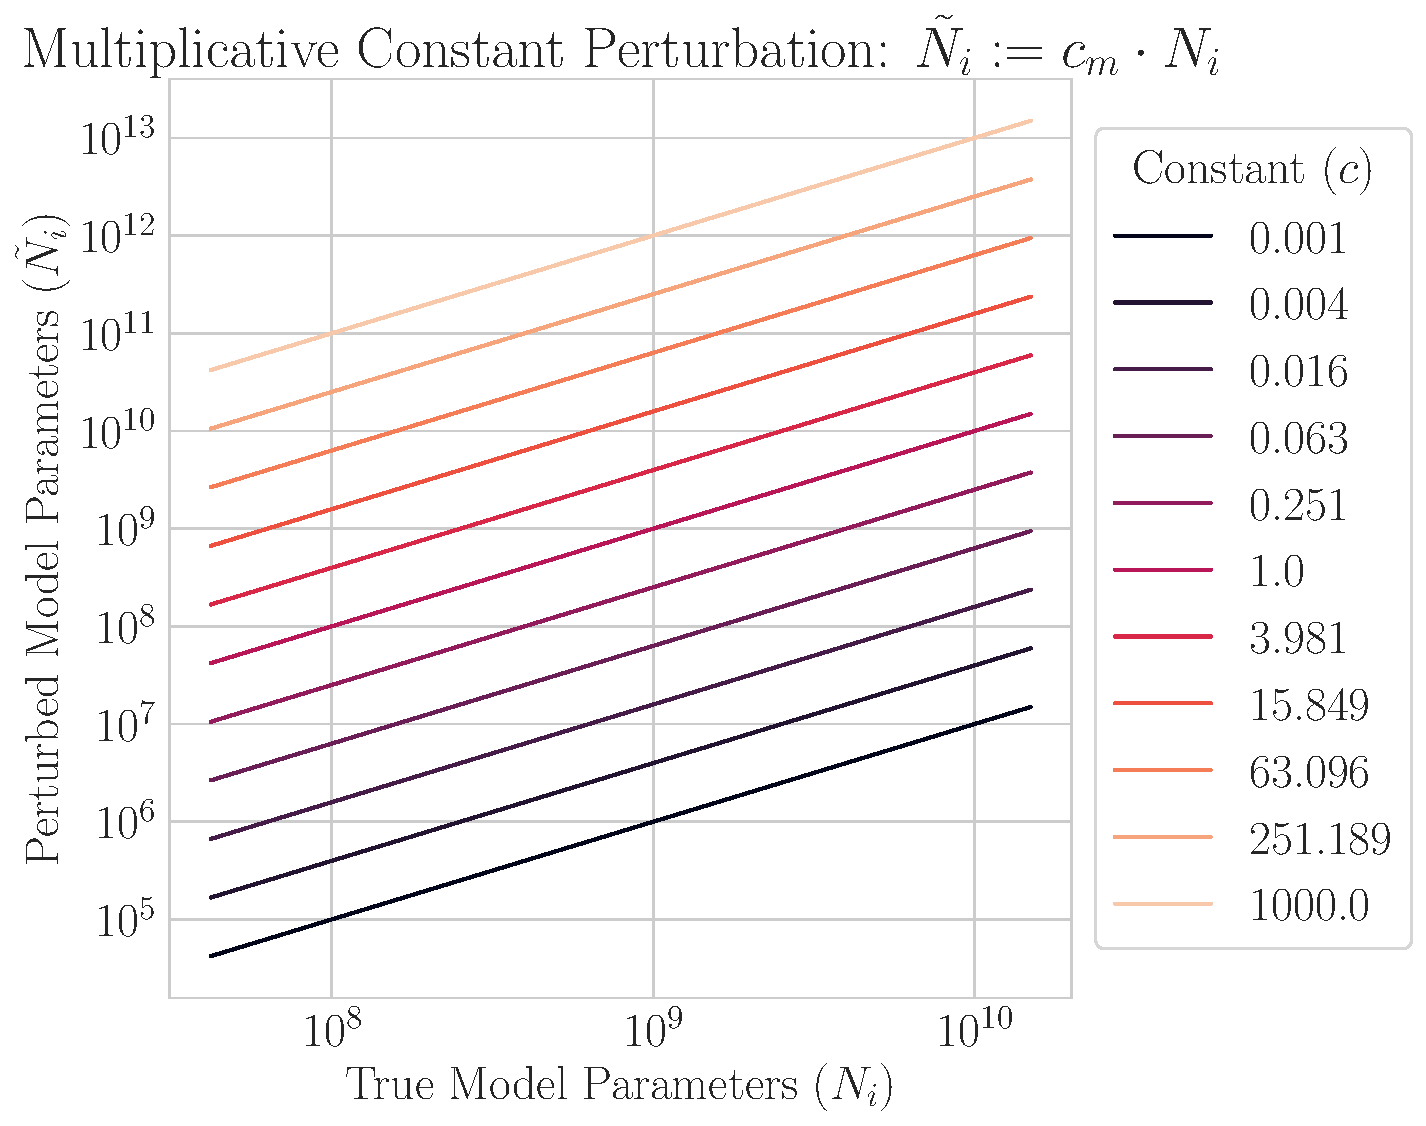
\includegraphics[width=0.46\linewidth]{figures/y=perturbed-params_x=params_multiplicative_constant.pdf}\hfill
    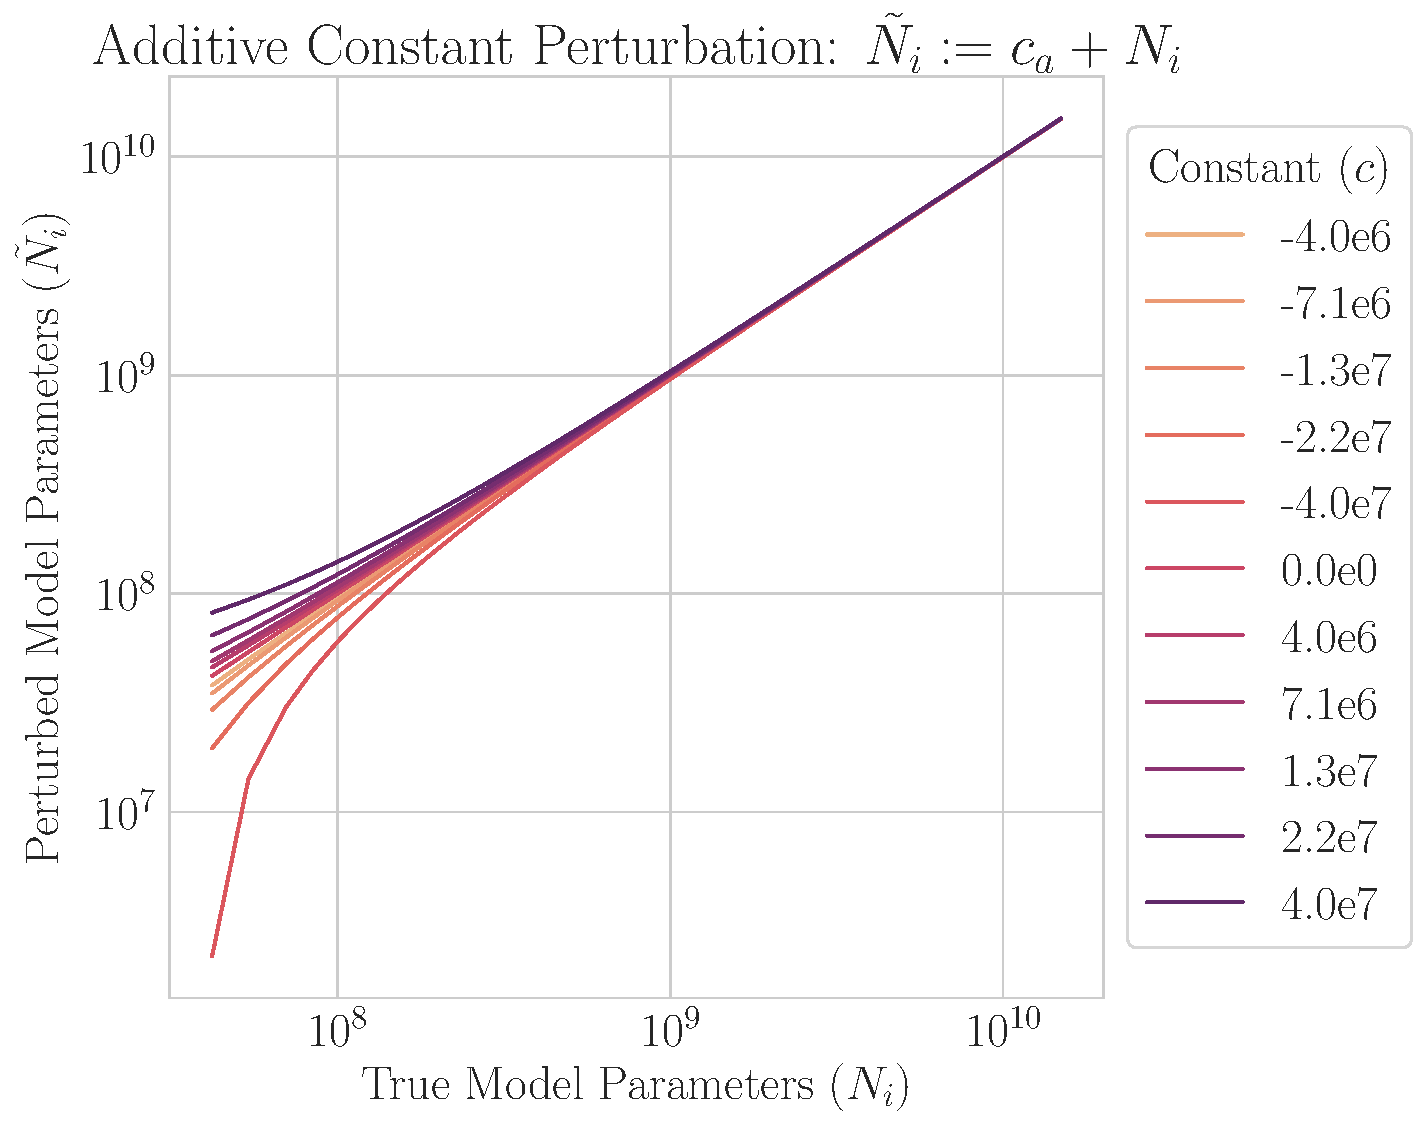
\includegraphics[width=0.46\linewidth]{figures/y=perturbed-params_x=params_additive_constant.pdf}
    \vspace{0.2cm} % Small gap
    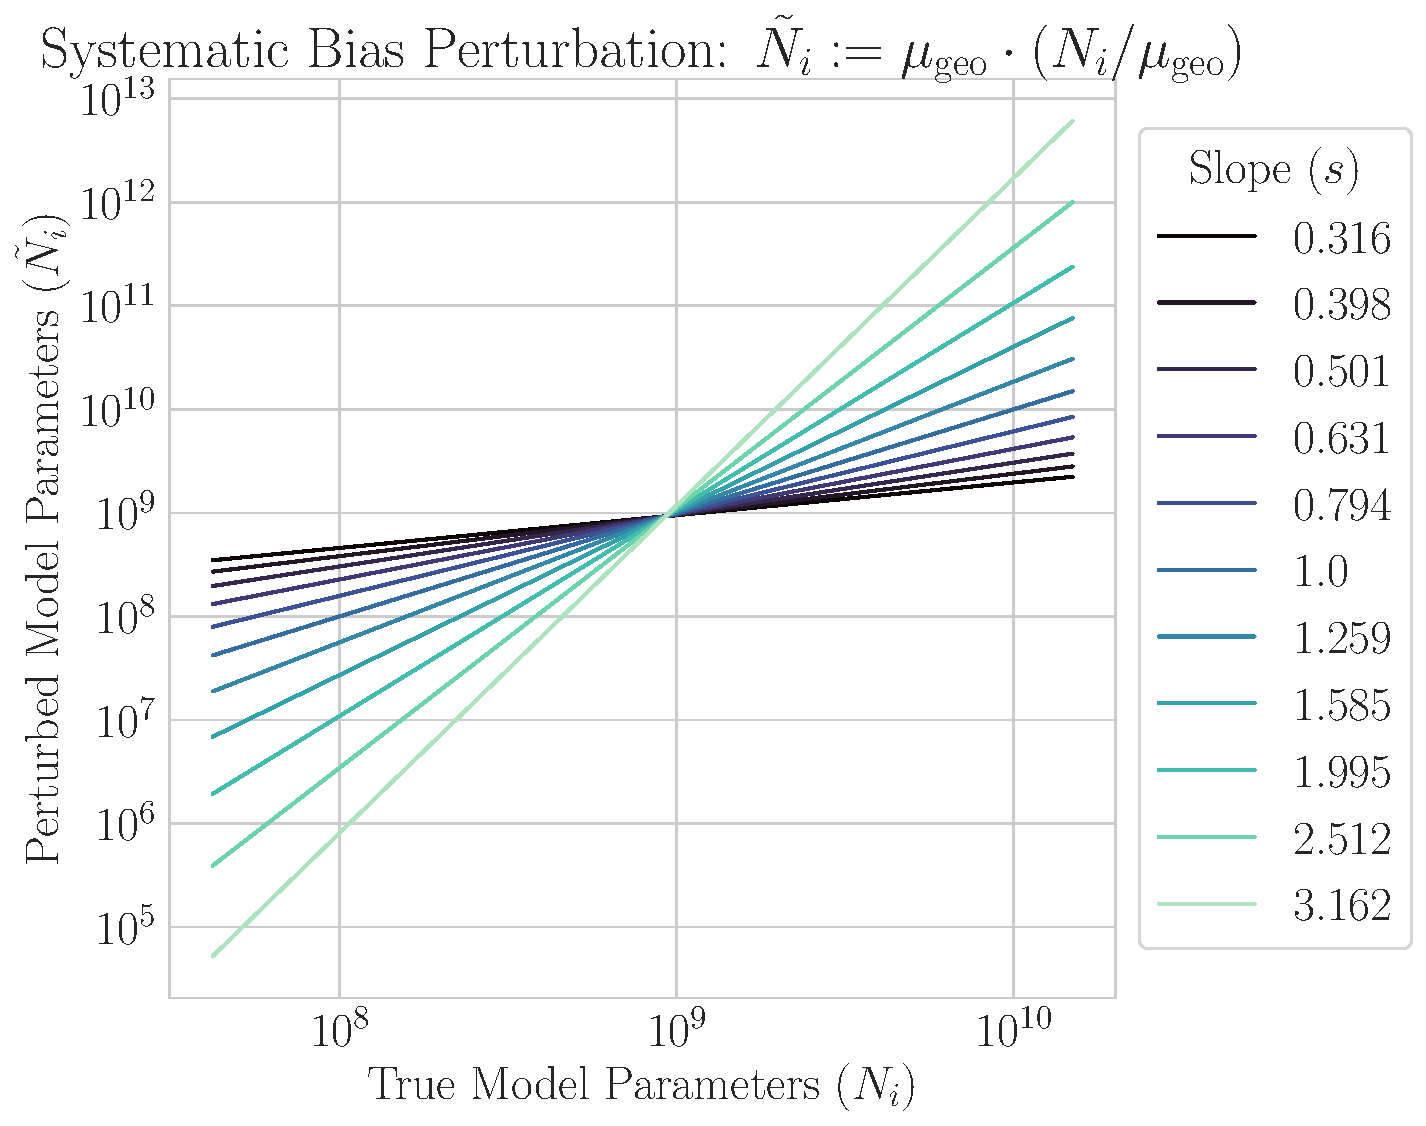
\includegraphics[width=0.46\linewidth]{figures/y=perturbed-params_x=params_systematic_bias.pdf}\hfill
    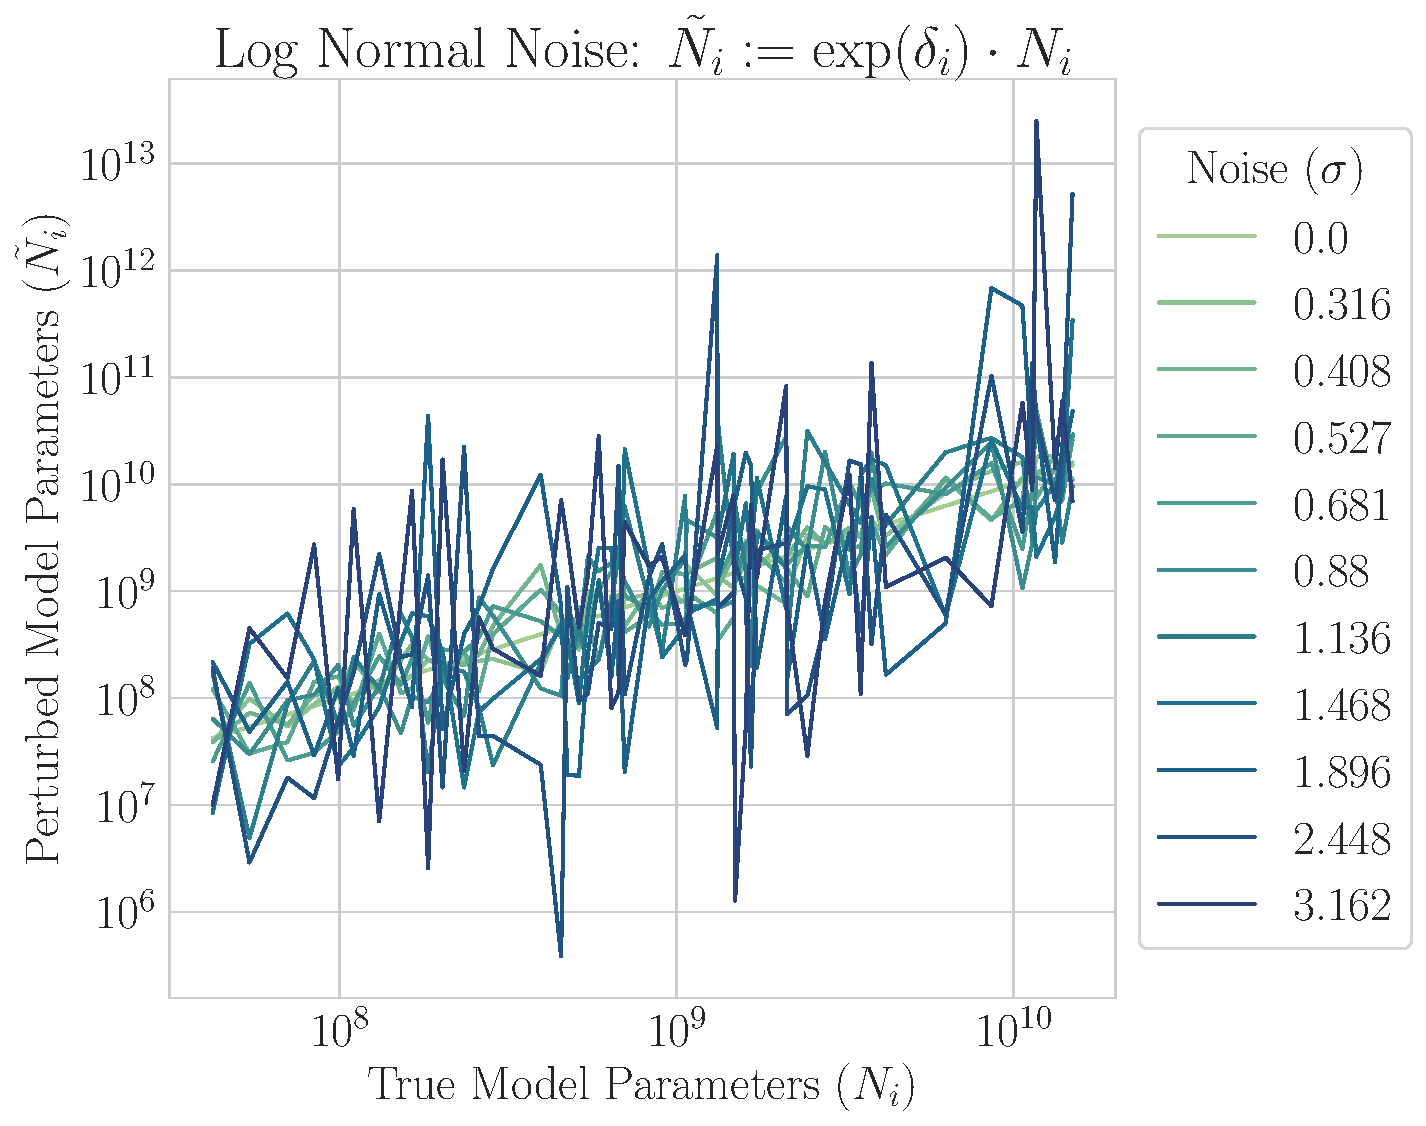
\includegraphics[width=0.46\linewidth]{figures/y=perturbed-params_x=params_log_normal_noise.pdf}
    \caption{\textbf{Evaluating the Robustness of Chinchilla via Four Model Parameter Perturbations.} We study how robust key Chinchilla results are to structured perturbations of models' parameters. \textbf{Top Left:} In the first perturbation, motivated by Sec.~\ref{sec:model_params_bestfit}, we perturb model parameters with a multiplicative constant $c_m$.
    \textbf{Top Right:} In the second perturbation, we perturb model parameters with an additive constant $c_a$, that could perhaps arise due to embedding parameters being included/excluded.
    \textbf{Bottom Left:} In the third perturbation, we perturb model parameters with a systematic bias: either smaller models' parameters are larger and larger models' parameters are smaller, or smaller models' parameters are smaller and larger models' parameters are larger; the systematic bias is controlled by slope $s$. \textbf{Bottom Right:} In the fourth perturbation, we assume the relationship of the loss with model parameters is perhaps noisy, e.g., \citep{frankle2019lottery}, with noise strength parameterized by $\sigma$.}
    \label{fig:perturbations_intuition}
\end{figure*}

\section{Robustness of Chinchilla Headline Results Depends on Type of Perturbation to Model Parameters}
\label{sec:robustness_analysis}

Given that the key Chinchilla results did not meaningfully change even when model parameters differed by as much as 15.2\%, we next asked:
%
\begin{quote}
\begin{center}
    \textit{How distorted could the model parameters have been without meaningfully affecting Chinchilla's headline results?}
\end{center}
\end{quote}
%
To answer this question, we intentionally perturbed the standard formula model parameters in four structured ways: multiplicative constant, additive constant, systematic bias and log normal noise. We then reran the fitting processes using the perturbed model parameters to see what effect each type of perturbation has on the estimated scaling law parameters and compute-optimal tokens-per-parameter.
We offer visual intuition for each of the four types of perturbations (Fig.~\ref{fig:perturbations_intuition}).

\subsection{Multiplicative Constant Perturbation Increases $\hat{A}$ Exponentially}
\label{sec:robustness_analysis:subsec:multiplicative_constant}

Motivated by Sec.~\ref{sec:model_params_bestfit}, for our first perturbation, we assume model parameters are systematically under/overestimated by approximately the same percentage.
To model this, we multiplied all true model parameters $\{N_i\}_i$ by constant multiplier $c_m$ to produce perturbed model parameters $\{\tilde{N}_i\}_i$:
%
\begin{equation}\label{eqn:multiplicative_constant}
    \Tilde{N}_i \defeq c_m \cdot  N_i .
\end{equation}
%
We swept $c_m$ in logspace(-3, 3, num=11). For visual intuition, see Fig.~\ref{fig:perturbations_intuition}, top left. 

% Removed \clearpage here to prevent whitespace gaps
% Switched to figure* to span two columns, preventing vertical overflow
\begin{figure*}[t]
    \centering
    \begin{subfigure}{0.48\textwidth}
        \centering
        \caption*{Multiplicative Constant: $\Tilde{N}_i \defeq c_m \cdot N_i$}
        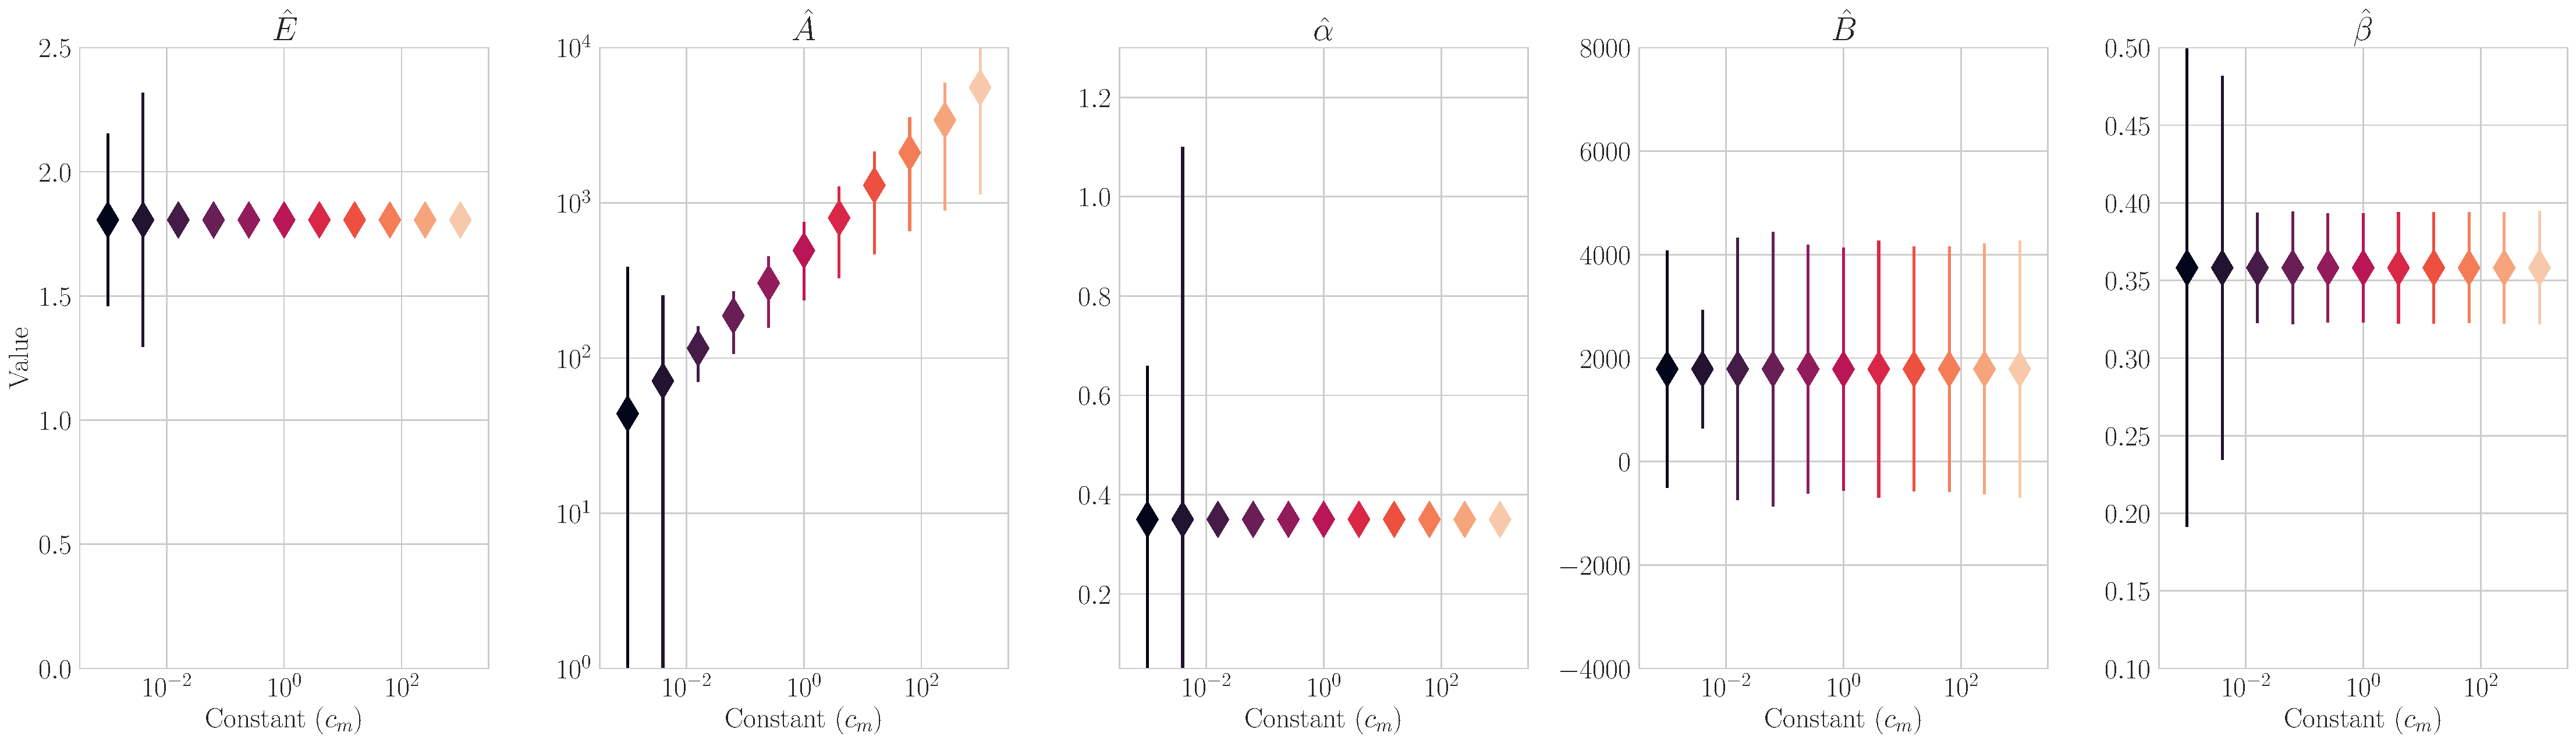
\includegraphics[width=\linewidth]{figures/fit_parameters_multiplicative_constant.pdf}
    \end{subfigure}\hfill
    \begin{subfigure}{0.48\textwidth}
        \centering
        \caption*{Additive Constant: $\Tilde{N}_i \defeq c_a + N_i$}
        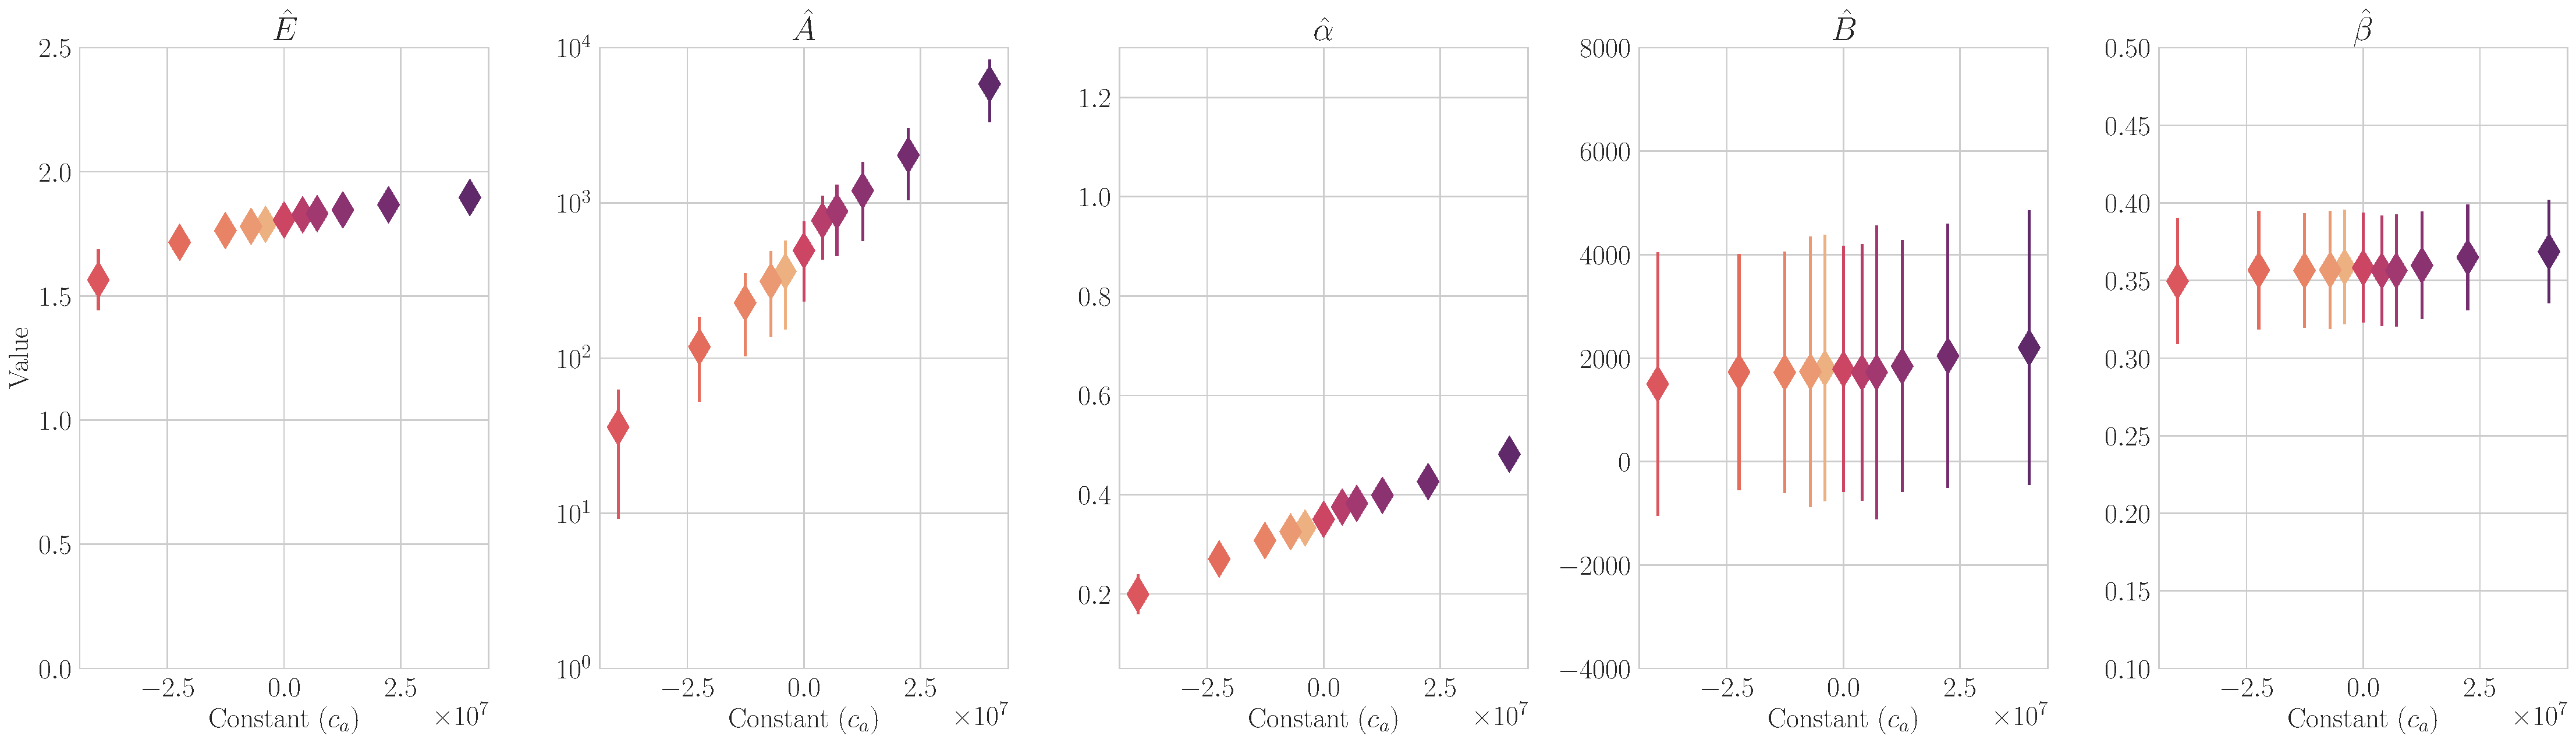
\includegraphics[width=\linewidth]{figures/fit_parameters_additive_constant.pdf}
    \end{subfigure}
    
    \vspace{0.4cm}
    
    \begin{subfigure}{0.48\textwidth}
        \centering
        \caption*{Systematic Bias: $\Tilde{N}_i \defeq \mu_{\mathrm{geo}} \cdot ( N_i / \mu_{\mathrm{geo}})^{s}$}
        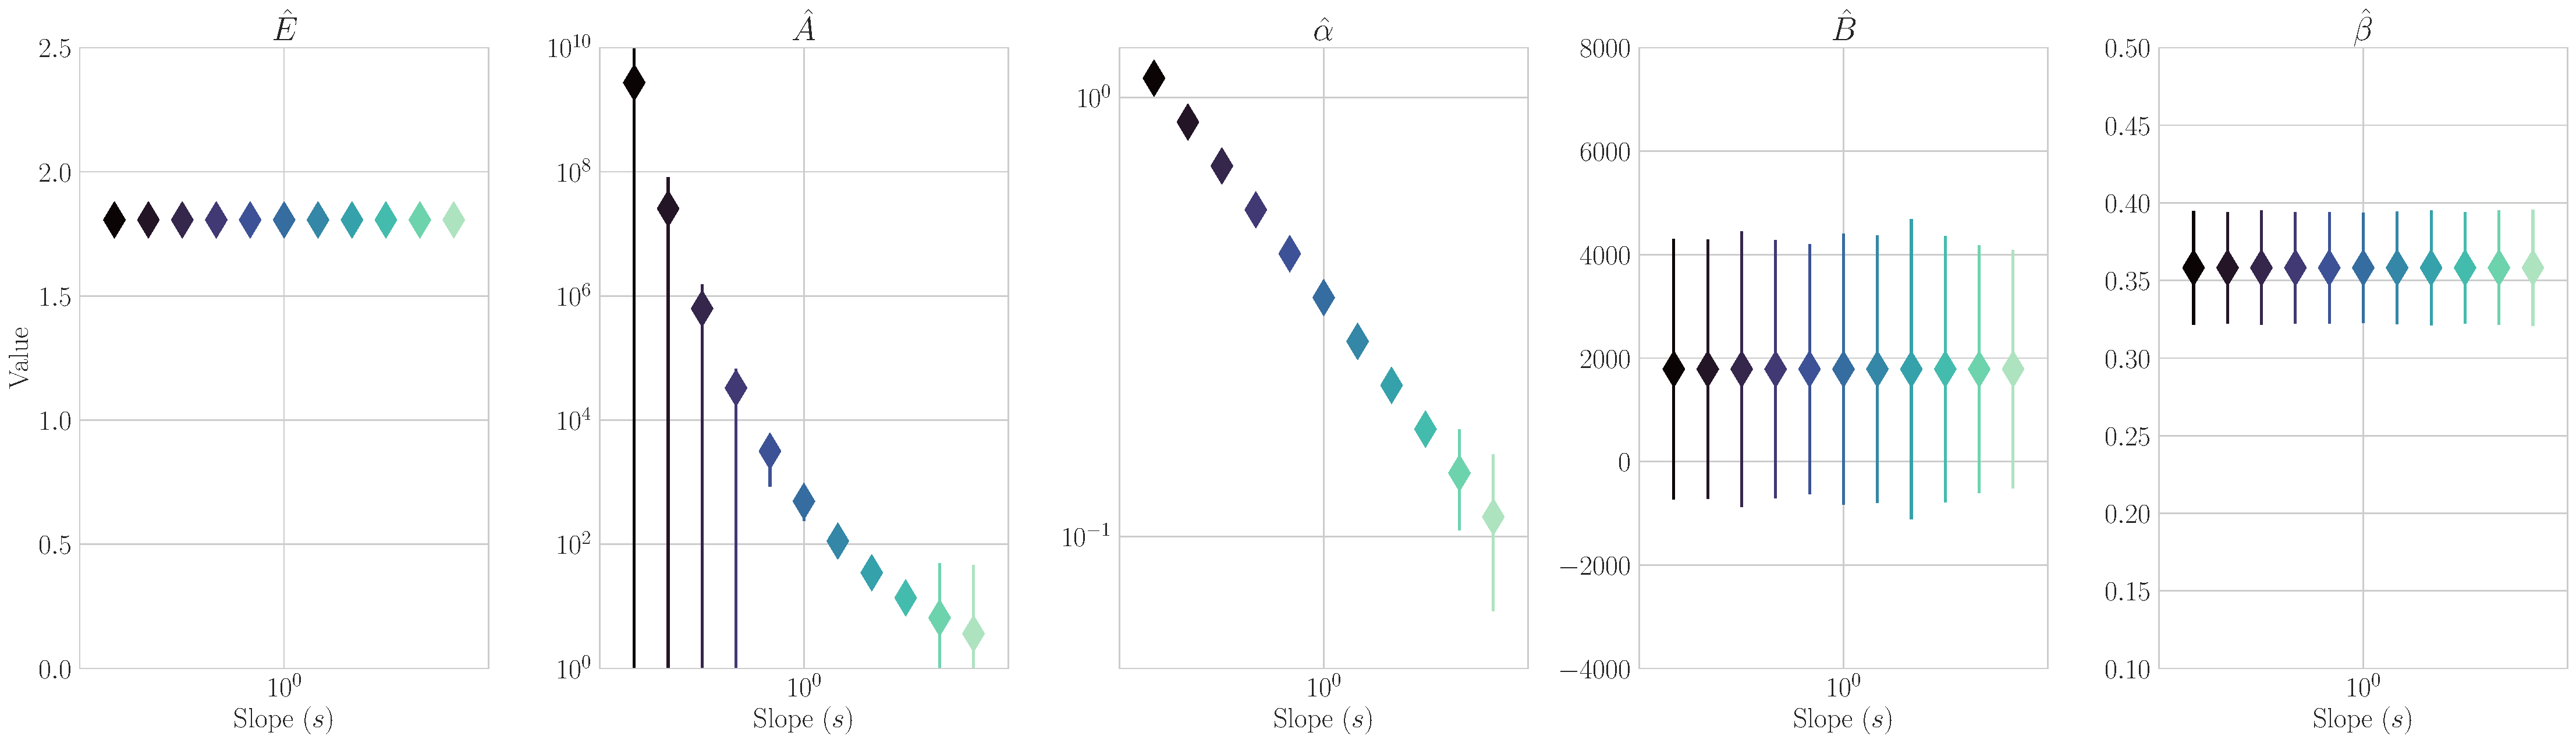
\includegraphics[width=\linewidth]{figures/fit_parameters_systematic_bias.pdf}
    \end{subfigure}\hfill
    \begin{subfigure}{0.48\textwidth}
        \centering
        \caption*{Log Normal Noise: $\Tilde{N}_i = \exp(\delta_i) \cdot N_i$}
        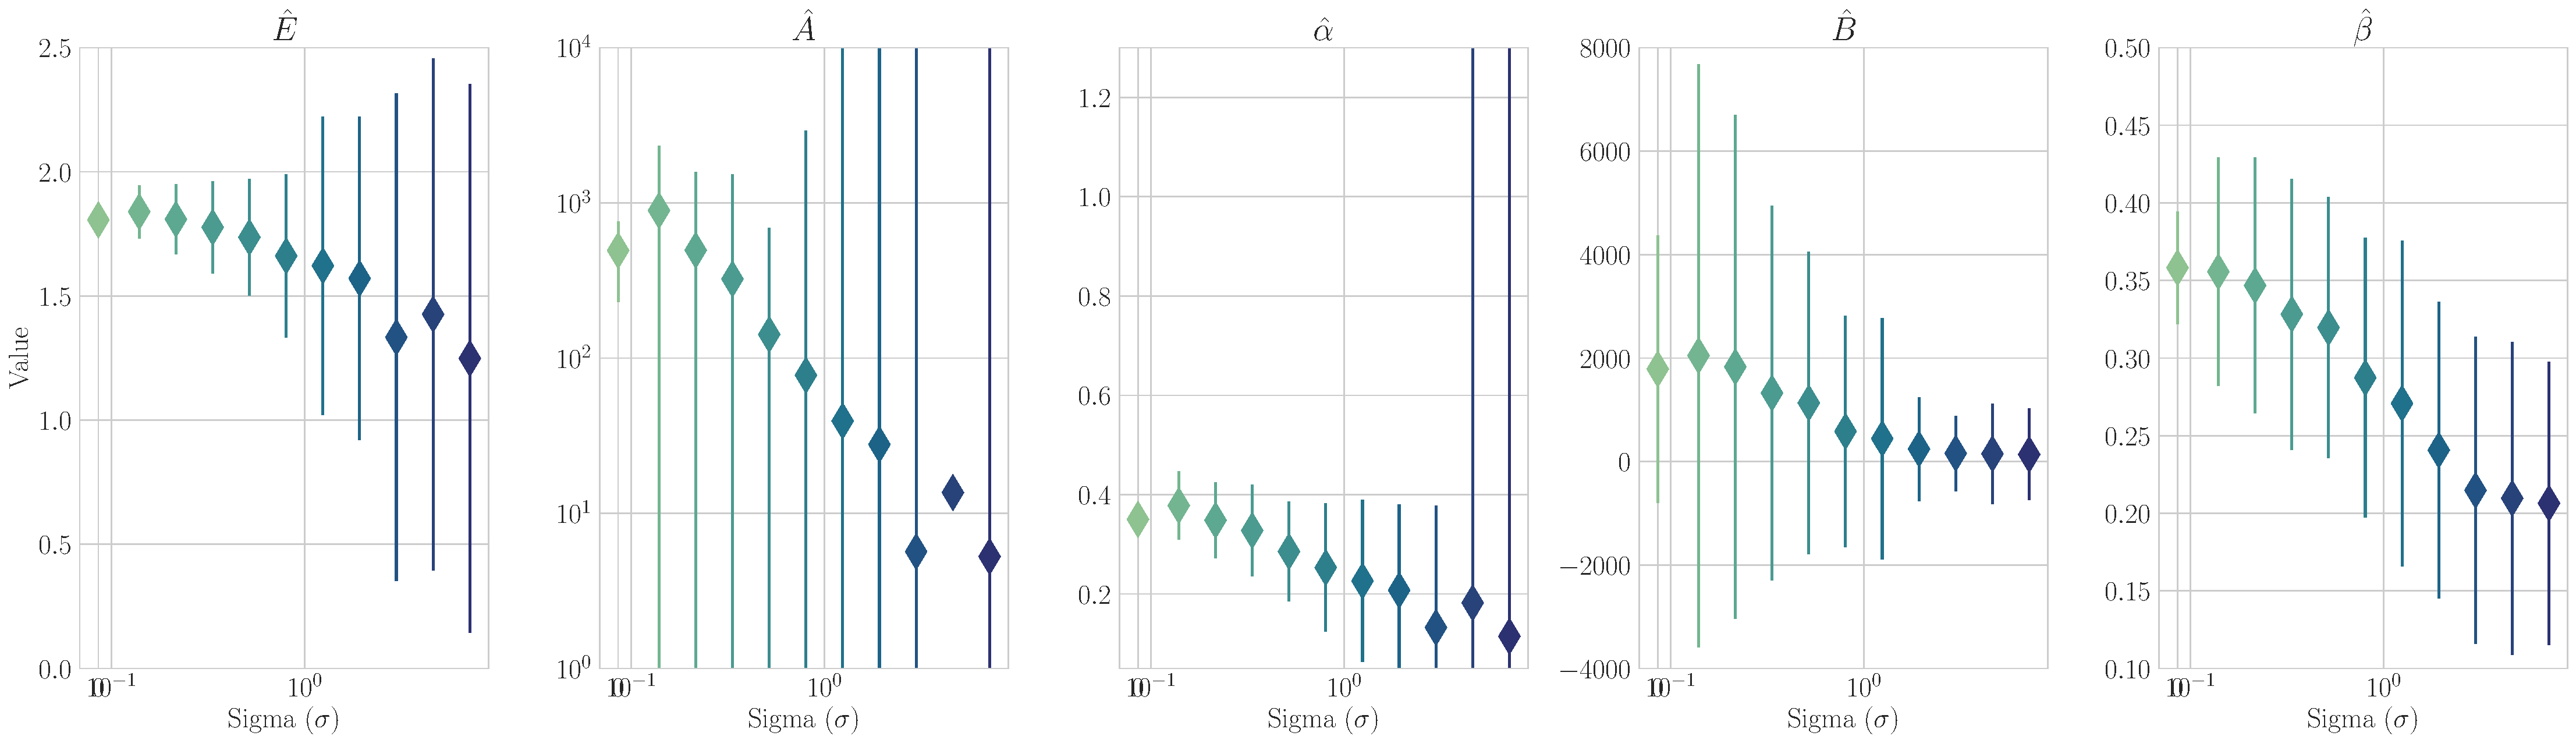
\includegraphics[width=\linewidth]{figures/fit_parameters_log_normal_noise.pdf}
    \end{subfigure}
    
    \caption{
    \textbf{Robustness of Fit Neural Scaling Law Parameters Under Four Types of Model Parameter Perturbations.}
    Each plot visualizes the effect of a different perturbation on the five fit parameters of the Chinchilla scaling law ($L(N,D) = E + A \cdot N^{-\alpha} + B \cdot D^{-\beta}$).
    \textbf{Top Left:} A multiplicative constant perturbation ($c$) increases the model parameter prefactor ($\hat{A}$) exponentially, while other fit parameters remain stable.
    \textbf{Top Right:} An additive constant perturbation ($c$) linearly increases the model parameter exponent ($\hat{\alpha}$) and exponentially increases its prefactor ($\hat{A}$), with only a gentle rise in the irreducible loss ($\hat{E}$).
    \textbf{Bottom Left:} A systematic bias perturbation ($s$) causes the model parameter exponent ($\hat{\alpha}$) to decay as a power law ($s^{-1}$) and the prefactor ($\hat{A}$) to decline sub-polynomially.
    \textbf{Bottom Right:} Adding log-normal noise ($\sigma$) primarily increases the uncertainty of all fit parameters, while weakly decreasing the model parameter exponent ($\hat{\alpha}$) logarithmically and the prefactor ($\hat{A}$) polynomially. Error bars are standard errors obtained by $4000$ bootstrapped samples.
    }
    \label{fig:perturbed_fits}
\end{figure*}

As we derive in Appendix~\ref{app:theoretical_analysis:subsec:multiplicative} and show empirically in Fig.~\ref{fig:perturbed_fits} (Top Left), the fitting process compensates for this multiplicative error primarily by adjusting the model size prefactor, $\Tilde{\hat{A}}$, to approximately $\hat{A} c_m^{\alpha}$, while the scaling exponent, $\hat{\alpha}$, remains largely unchanged, i.e., $\Tilde{\hat{\alpha}} \approx \hat{\alpha}$.
This makes sense for moderate $c_m$: if $\hat{A}$ is the best fit for the true model parameters, then replacing the true parameters with the perturbed parameters $N_i \rightarrow \tilde{N}_i$ and rescaling $\hat{A} \rightarrow \Tilde{\hat{A}} = (c_m)^{\alpha} \hat{A}$ produces approximately the same fit.
As a consequence, Fig.~\ref{fig:perturbed_compute_optimal_tpp} Top Left shows the compute-optimal tokens per parameter remains constant with pretraining compute, but the precise constant grows as a power of $c_m$ if true model parameters are underestimated $(c_m < 1)$ and shrinks if true model parameters are overestimated $(c_m > 1)$.
The only exceptions are for the two smallest multiplicative constants ($0.001$ and $0.004$), where uncertainty in $\hat{A}$ and $\hat{\alpha}$ produced \texttt{NaNs}.

\subsection{Additive Constant Perturbation Increases $\hat{\alpha}$ Linearly and $\hat{A}$ Exponentially}
\label{sec:robustness_analysis:subsec:additive_constant}

In our second perturbation, we assume model parameters have an additive term. For example, embedding parameters may be included or excluded, a key detail in previous scaling law studies \citep{kaplan2020scaling, hoffman2022chinchilla} that is partially responsible for discrepancies between estimated scaling laws' parameters \citep{pearce2024reconciling, porian2024resolvingdiscrepancies}). To model this, we added constant $c_a$ to all model parameters:
%
\begin{equation}\label{eqn:additive_constant}
    \Tilde{N}_i \defeq c_a +  N_i .
\end{equation}
%
We swept $c_a$ in -logspace(6.6, 7.6, num=5) $\cup \, \{0\} \, \cup $ logspace(6.6, 7.6, num=5). For visual intuition, see Fig.~\ref{fig:perturbations_intuition} Top Right. For additional context, the smallest Chinchilla model has $42\times10^6$ parameters.

Fig.~\ref{fig:perturbed_fits} (Top Right) shows the effects:
\emph{(i)}~the irreducible loss $\hat{E}$ rises only gently from $1.565$ to $1.897$ ($\approx 21\%$).
\emph{(ii)}~the model parameter prefactor $\hat{A}$ grows exponentially in $c_a$, increasing by $\sim\!2.5x$ from the most negative to the most positive constant
\emph{(iii)}~the model parameter exponent $\hat{\alpha}$ increases linearly with $c_a$ from $0.199$ to $0.481$
and \emph{(iv)}~both the data prefactor $\hat{B}$ and data exponent $\hat{\beta}$ fluctuate only within their bootstrap error bars and show no systematic trend.
As a consequence, Fig.~\ref{fig:perturbed_compute_optimal_tpp} Top Right shows the compute-optimal tokens per parameter becomes less constant with the training compute: a larger positive $c_a$ means larger target training horizons require more tokens per parameter, whereas a larger negative $c_a$  means larger target training horizons require fewer tokens per parameter.

In Appendix~\ref{app:theoretical_analysis:subsec:additive}, we analytically explain these trends: the most critical parameter in a power law is its exponent, which corresponds to its slope in log-log space.
However, for the perturbed function, the slope is now no longer constant and depends on $N$ as $N/(N + c_a)$.
Thus, the fitting procedure must select a single exponent that best represents the varying slope over the range of data.
When $c_a > 0$, the factor $N/(N+c_a) < 1$, and the fitting process must select an exponent $\Tilde{\hat{\alpha}} > \hat{\alpha}$; and when $c_a < 0$, the factor $N/(N+c_a) > 1$, and to compensate, the fitting process must select an exponent $\Tilde{\hat{\alpha}} < \hat{\alpha}$.

For comparison, \citet{porian2024resolvingdiscrepancies} found that including the model's head parameters increased the fit model parameter scaling exponent $\hat{\alpha}$ by $0.080 \, (0.072 \rightarrow 0.152)$, and \citet{pearce2024reconciling} found that including embedding parameters increased $\hat{\alpha}$ by $0.231 \, (0.135 \rightarrow 0.366)$.
Although assuming an additive constant is a simplification of both analyses, all three results are quantitatively similar.

\subsection{Systematic Bias Perturbation Decreases $\hat{\alpha}$ Polynomially and $\hat{A}$ Sub-Polynomially}
\label{sec:robustness_analysis:subsec:systematic_bias}

In our third perturbation, we assume the presence of a systematic bias in reported models' parameters: either the smaller models' parameters are truly larger and the larger models' parameters truly smaller, or vice versa.
To model this, we define the perturbed parameters as
%
\begin{equation}\label{eqn:systematic_bias}
    \tilde{N}_i \defeq \mu_{\mathrm{geo}} \cdot \left( N_i \, / \, \mu_{\mathrm{geo}} \right)^{s},
\end{equation}
%
where \(\mu_{\mathrm{geo}} \defeq (\prod_i N_i)^{1/\text{Num. Models}}\) is the geometric mean of the model parameters and \(s\) is the systematic bias parameter: \(s < 1\) shrinks large models and inflates small ones, whereas \(s > 1\) does the reverse.
We swept $s$ in logspace(-0.5, 0.5, 11). For visual intuition, see Fig.~\ref{fig:perturbations_intuition} Bottom Left.

Fig.~\ref{fig:perturbed_fits} (Bottom Left) illustrates three main effects:
\emph{(i)}~The model parameter exponent $\hat{\alpha}$ decays according to the power-law relationship $\hat{\alpha} = 10^{-0.46} \cdot s^{-1}$, which is a nearly perfect fit to the data ($R^2 > 0.999$, $p \approx \num{5.9e-90}$).
\emph{(ii)}~The model parameter prefactor $\hat{A}$ declines sub-polynomially.
\emph{(iii)}~The irreducible loss, $\hat{E}$, and the data parameters, $\hat{B}$ and $\hat{\beta}$, show no systematic trend, with fluctuations remaining within their bootstrap error bars.
Similar to the Additive Constant perturbation, Fig.~\ref{fig:perturbed_compute_optimal_tpp} Bottom Left shows that the two trends of $\hat{A}$ and $\hat{\alpha}$ together make the compute-optimal tokens per parameter ratio less constant with the target training horizon: a larger systematic bias $s$ means larger target training horizons require fewer tokens per parameter, whereas a smaller systematic bias $s$  means larger target training horizons require more tokens per parameter.

\begin{figure*}[t]
    \centering
    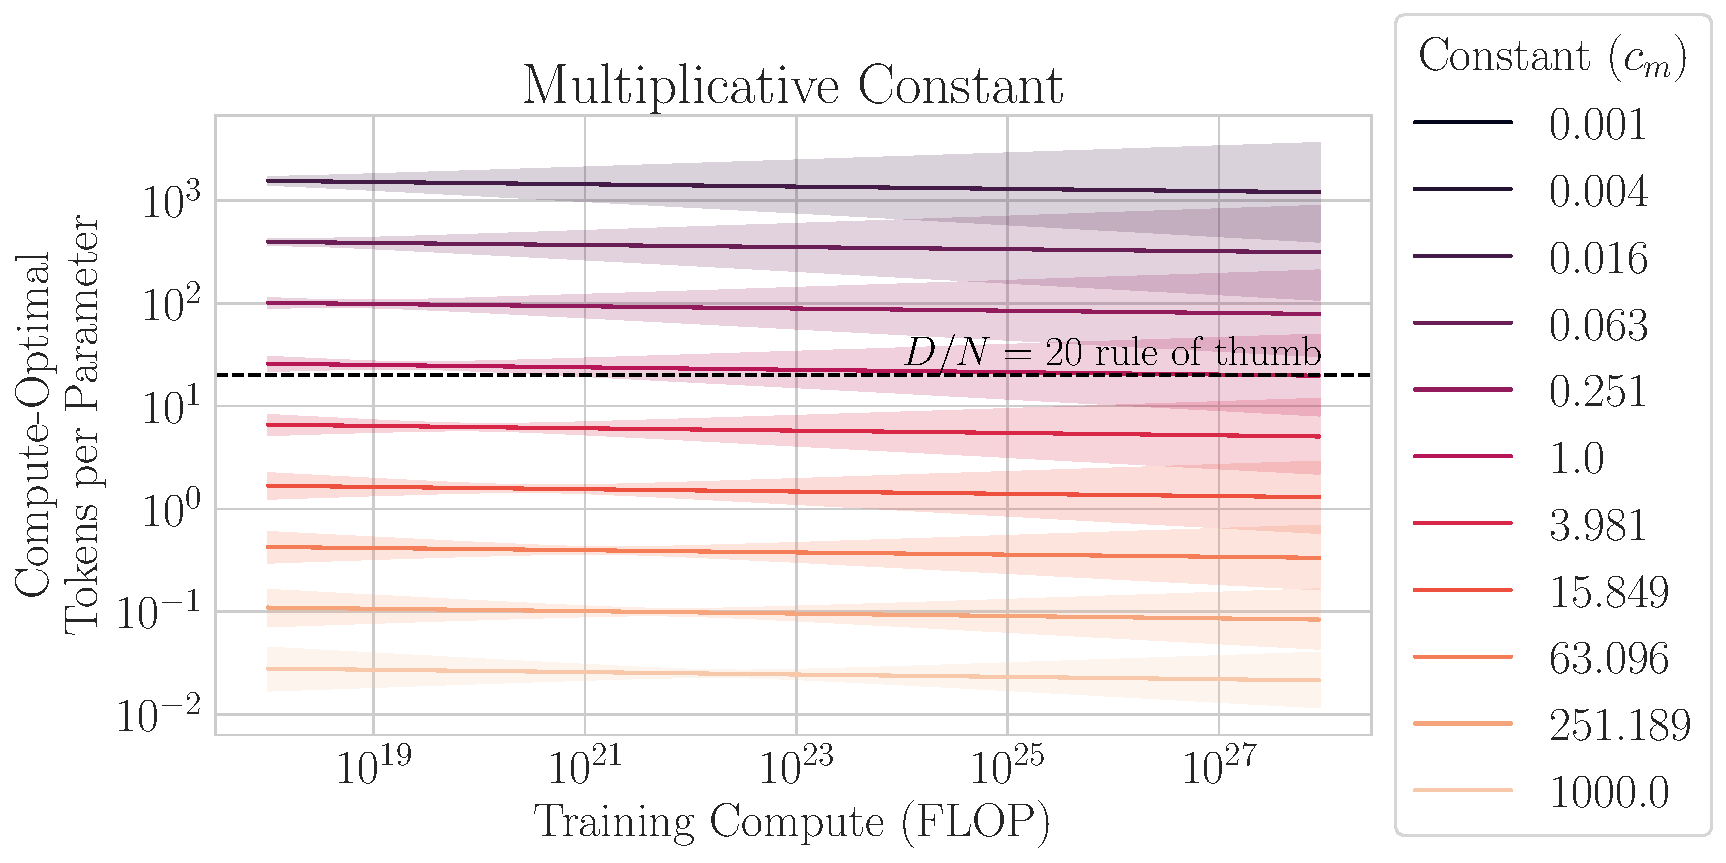
\includegraphics[width=0.48\linewidth]{figures/compute_optimal_tokens_per_parameter_by_compute_multiplicative_constant.pdf}%
    \hfill
    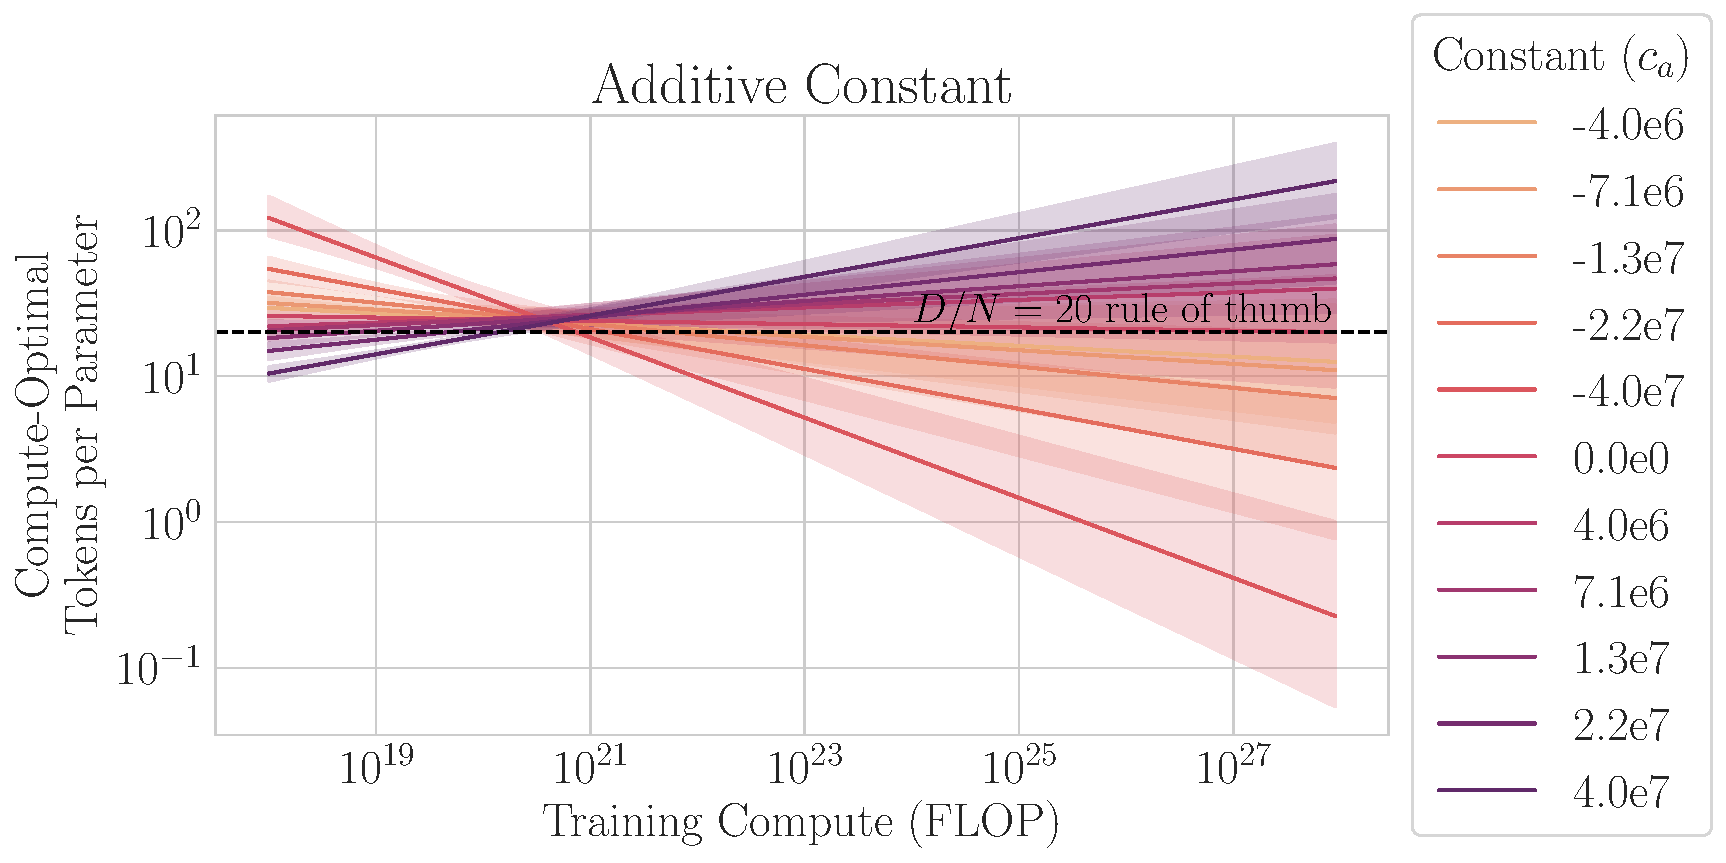
\includegraphics[width=0.48\linewidth]{figures/compute_optimal_tokens_per_parameter_by_compute_additive_constant.pdf}
    \vspace{0.2cm}
    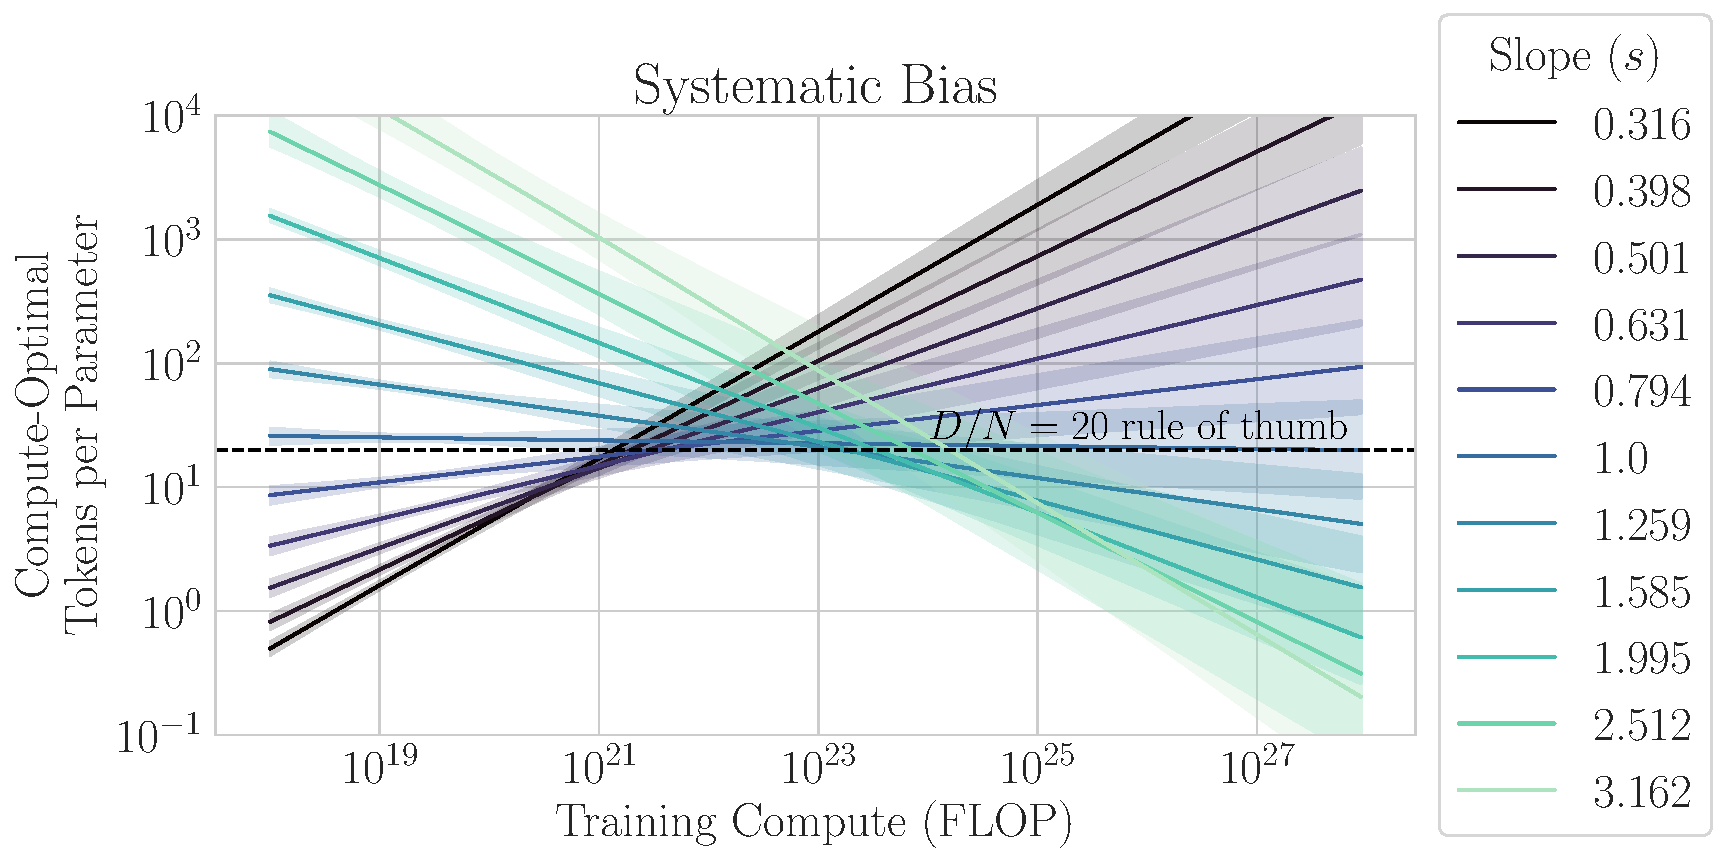
\includegraphics[width=0.48\linewidth]{figures/compute_optimal_tokens_per_parameter_by_compute_systematic_bias.pdf}%
    \hfill
    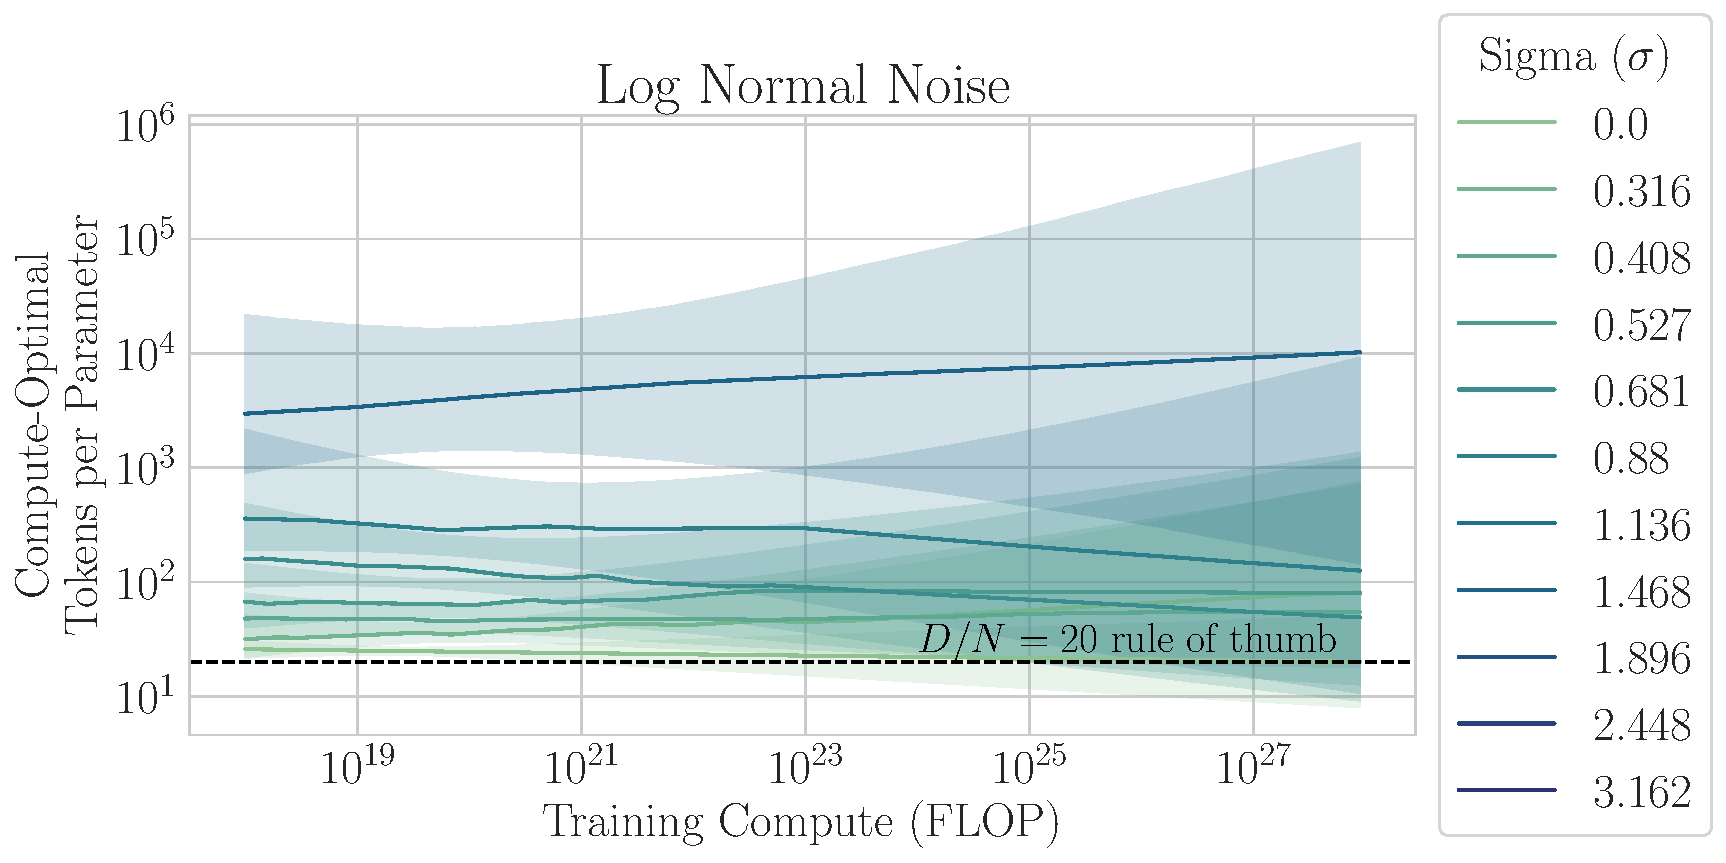
\includegraphics[width=0.48\linewidth]{figures/compute_optimal_tokens_per_parameter_by_compute_log_normal_noise.pdf}
    \caption{
    \textbf{Robustness of Compute-Optimal Tokens-Per-Parameter Under Four Types of Model Parameter Perturbations.} 
    Shaded regions represent 80\% confidence intervals.
    \textbf{Top Left:} A multiplicative constant perturbation by $c$ shifts the compute-optimal ratio by $c^{\alpha}$ but keeps the trend flat with respect to training compute.
    \textbf{Top Right:} An additive constant perturbation by $c$ makes the compute-optimal ratio less constant across the target training compute horizon. A positive slope means more tokens are needed per parameter for larger compute budgets, while a negative slope means fewer are required. 
    \textbf{Bottom Left:} A systematic bias also makes the ratio less constant. A larger bias $(s > 1)$ leads to fewer optimal tokens per parameter for larger models, whereas a smaller bias $(s < 1)$ requires more. 
    \textbf{Bottom Right:} Adding log-normal noise to model parameters increases the uncertainty and the overall magnitude of the compute-optimal tokens per parameter ratio.
    }
    \label{fig:perturbed_compute_optimal_tpp}
\end{figure*}

In Appendix~\ref{app:theoretical_analysis:subsec:systematic}, we mathematically derive that under the systematic bias, the model parameter exponent is multiplied by $s^{-1}$ and the model prefactor is multiplied by $\mu_{\mathrm{geo}}^{\alpha(1-s)/s}$, making the exponent in the compute-optimal ratio $(\alpha/s - \beta) / (\alpha/s + \beta)$. Thus, if $s < 1$, then the exponent on $C$ becomes positive and compute-optimal ratio of tokens-per-parameter increases with compute, whereas if $s > 1$, then the exponent on C becomes negative and the compute-optimal ratio of tokens-per-parameter decreases with compute.


\subsection{Log Normal Noise Perturbation Increases Uncertainty and Decreases $\hat{\alpha}$ Logarithmically and $\hat{A}$ Polynomially}
\label{sec:robustness_analysis:subsec:log_normal_noise}

In our fourth perturbation, we assume the ``value'' of model parameters is noisily measured, perhaps due to model initializations. To model this, we added log-normal noise to the number of parameters. Specifically, for each model's parameter count $N_i$, we sampled a new parameter count as:
%
\begin{equation}\label{eqn:log_normal_noise}
    \Tilde{N}_i \defeq \exp(\delta_i) \cdot N_i , \quad \quad  \delta_i \sim \mathcal{N}(0, \sigma^2).
\end{equation}
We swept $\sigma$ from $\num{1e-2}$ to $\num{1e2}$. For visual intuition, see Fig.~\ref{fig:perturbations_intuition} Bottom Right.

Fig.~\ref{fig:perturbed_fits} (Bottom Right) illustrates three main effects:
\emph{(i)}~Nearly all fit parameters have significantly larger confidence intervals, especially as the noise standard deviation $\sigma$ increases; for the highest value of $3.162$, $\hat{A}$ and $\hat{\alpha}$ are nearly unidentifiable.
\emph{(ii)}~To the extent that trends can be identified, the irreducible error $\hat{E}$ trends down weakly, while the model parameters prefactor $\hat{A}$ falls roughly polynomially and the model parameters exponent falls roughly logarithmically with the noise standard deviation $\sigma$.
Fig.~\ref{fig:perturbed_compute_optimal_tpp} Bottom Right demonstrates the consequences of the noise: fits with too high of noise create NaNs, while noise drives up the compute-optimal tokens per parameter and also increases the width of the 80\% confidence intervals by $\sim 1$ order of magnitude, although the inferred values are roughly constant with target training compute.